\section{模型实验}
\label{sec:model}

\subsection{实验框架的实现}

本次实验框架主要使用的是Python的sklearn包进行实现的。此外,还使用了Python的xgboost包。后者的模型也进行了sklearn的封装,因此我们可以编写统一的实验框架。我们使用的实验框架中,使用的模型、特征文件、特征列表、模型参数等等都可以以命令行参数的形式进行指定。这样,在实验时,我们不需要修改训练模型的代码,只需要修改命令就行了。同时,通过记录命令的详细内容和每次实验的中间结果,我们可以很方便地对实验过程进行总结,比较特征的能力,并把模型调到最优的表现。

\subsection{K最近邻}

这部分,我们首先对于前面在\ref{subsec:feature4}中设计的四维空间数据点进行简单探索。我们使用KNN模型,以四维时空数据点作为训练数据进行交叉验证测试,观察做数据标准化的效果。我们对数据统一进行3000邻居的KNN预测,标准化之前的交叉验证结果为2.67,标准化之后的交叉验证结果提升到了2.62。说明数据标准化确实是有利的。但是,现在的效果还有提升的空间:我们可以进一步调整时间、空间特征差异的权重(现在二者的权重是一样的),强调某一些更重要的特征,这样可能能用KNN得到更好的结果。

\subsection{随机森林}

由于随机森林的训练也测试速度比较快,因此我们使用随机森林模型来比较不同特征的预测能力。使用的特征有:

\begin{itemize}
    \item \textbf{特征0:}直接对原始数据文件数值化之后的特征,其构造方法为第\ref{subsec:feature0}节中的描述。
    \item \textbf{特征3:}在特征0的基础上,加入街道特征。街道特征的构造方法为第\ref{subsec:feature3}节中的描述。
    \item \textbf{特征4:}在特征0的基础上,加入时空数据点的K最近邻特征。K最近邻特征的构造方法为第\ref{subsec:feature4}节中的描述。
    \item \textbf{特征5:}在特征0的基础上,加入空间坐标的聚类结果特征。聚类结果特征的构造方法为第\ref{subsec:feature5}节中的描述。
\end{itemize}

实验中,我们对随机森林使用两组参数:

\begin{itemize}
    \item \textbf{小规模随机森林:}使用更少的树,每棵树的规模也更小。具体为:30棵树,树的最大深度为8,叶子最少有80个样本。
    \item \textbf{大规模随机森林:}使用更多的树,每棵树的规模也更大。具体为:300棵树,树的最大深度为15,叶子最少有30个样本。
\end{itemize}

    \begin{table}[hb]
    \centering
    \caption{随机森林比较各种特征}
    \label{tb:rf}
    \begin{tabular}{|c|c|c|c|}
    \hline
    特征编号               & 模型参数 & 交叉验证结果 & 提交结果 \\ \hline
    \multirow{2}{*}{0} & 小规模  & 2.42   & 2.45 \\ \cline{2-4} 
                       & 大规模  & 2.29   & 2.30 \\ \hline
    \multirow{2}{*}{3} & 小规模  & 2.31   & -    \\ \cline{2-4} 
                       & 大规模  & 1.82   & 2.37 \\ \hline
    \multirow{2}{*}{4} & 小规模  & 2.27   & -    \\ \cline{2-4} 
                       & 大规模  & 2.03   & 2.49 \\ \hline
    \end{tabular}
\end{table}

表\ref{tb:rf}中展示了我们使用随机森林测试不同特征的结果。首先可以看到的是,规模更大的随机森林能够得到更好的预测效果。但是,在增加了我们编制的特征之后,发生了比较令人费解的现象:虽然交叉验证的结果出现了巨大的提升,但是提交之后,在测试集上的结果却变差了。首先,既然能够在交叉验证时看到预测效果的提升,这可以说明我们编制特征的方法有一定效果。但是,发生了在训练集上效果好,而在测试集上效果远远更差的情况。显然,我们的特征发生了过拟合。推测的原因是,同一周之内的犯罪信息对于预测的影响过大。

为了验证这个想法,我们将训练集分为两折重新编制特征3,分折的方法仍然为隔周划分(奇数周为第1折,偶数周为第2折)。第1折的街道特征,使用第2折的街道信息进行统计和计算;第2折的街道特征,使用第1折的街道信息进行统计和计算。通过这种方式可以保证每一个数据点的特征,都没有参考同一周的数据进行计算。此时得到的结果见表\ref{tb:rf_3}。首先可以看到,测试集的结果和训练集比较接近了,这是一个很好的标志。但是,对比表\ref{tb:rf}中的结果可以发现,此时的预测结果仍然劣于原始的特征0。此外值得注意的是,使用一半数据编制的街道特征在测试集上的表现和使用全部数据的表现几乎一致。由此我们可以推断,使用全部时间段内的街道犯罪类型分布,对于随机森林可能只有负面的效果。

那么,为什么表\ref{tb:rf}中特征3的交叉验证结果会格外优秀呢?我们推测,这是因为在统计街道犯罪类型分布时,我们并没有包含每个数据点本身。于是,在预测时,如果发现某一类的概率比别的样本都小一点点,那么这个样本很可能属于这个类。所以,在编制特征3时,我们无形中提示了该样本的类型。正因如此,我们才在训练集上看到了一个格外好的假象(在测试集上才能看到这一特征的真正表现)。

\begin{table}[tb]
    \centering
    \caption{分折编制街道特征后的结果}
    \label{tb:rf_3}
    \begin{tabular}{|c|c|c|c|}
    \hline
    特征编号               & 模型参数 & 交叉验证结果 & 提交结果 \\ \hline
    \multirow{2}{*}{3(分折)} & 小规模  & 2.44   & -    \\ \cline{2-4} 
                       & 大规模  & 2.38   & 2.37 \\ \hline
    \end{tabular}
\end{table}

此外,我们也利用训练出的随机森林模型,对各个特征的重要程度进行了分析,结果如图\ref{fig:importance}。其中的大多数结果比较容易理解,比如地点坐标的重要性很高。根据第\ref{sec:observation}节中对时间特征的分析,我们也可以理解年份和小时都是比较重要的。但是,比较令人费解的是,分钟成为了重要性最高的特征。我们尝试给出的解释是,犯罪记录中的时间并不是犯罪真正发生的具体时刻,而是该次犯罪录入档案的时刻。在记录的过程中,可能在不同犯罪类型之间,人为引入了令人意想不到的差别。此外,两个街道特征的重要性差别,应该是在第\ref{subsec:feature0}部分中,对街道地址的编码方式引入的。

\begin{figure}[tb]
    \centering
    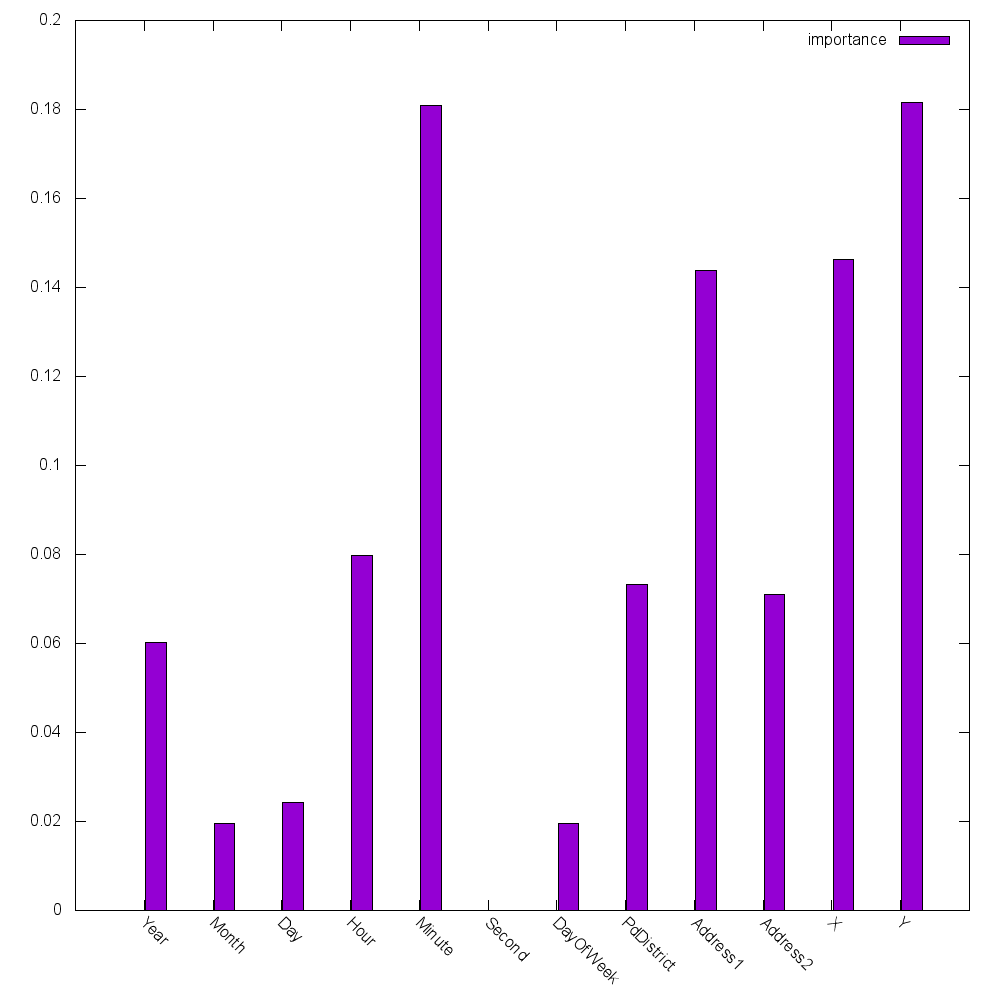
\includegraphics[width=1.0\linewidth]{fig/importance}
    \caption{特征重要性}
    \label{fig:importance}
\end{figure}

\subsection{Xgboost}

我们最终提交的结果是Xgboost跑出的结果,Xgboost在本次竞赛中相比其它我们使用的模型效果要出色很多。
表\ref{tb:xgboost}中是我们各次提交(各种参数配置下)的结果。

\begin{table*}[tb]
    \centering
    \caption{XgBoost调参过程}
    \begin{tabular}{|c|c|c|c|c|c|c|c|c|}
    \hline
    提交编号 & 使用特征编号 & 迭代轮数 & 决策树最深宽度 & 学习率 & 每棵树的列采样率 & 提交保留小数位数 & 交叉验证结果 & 提交结果 \\
    \hline
    1 & 0 & 60 & 8 & 0.3 & 1 & 3 & 2.22376 & 2.31334 \\
    \hline
    2 & 0 & 100 & 8 & 0.1 & 1 & 3 & 2.259029 & 2.29657 \\
    \hline
    3 & 0 & 100 & 10 & 0.1 & 1 & 3 & 2.235178 & 2.29852 \\
    \hline
    4 & 0 & 100 & 6 & 0.1 & 1 & 3 & 2.289943 & 2.31782 \\
    \hline
    5 & 0 & 200 & 6 & 0.1 & 1 & 3 & 2.263382 & 2.31364 \\
    \hline
    6 & 4 & 200 & 6 & 0.1 & 1 & 3 & 2.208462 & 2.64618 \\
    \hline
    7 & 3 & 200 & 6 & 0.1 & 1 & 3 & 2.24326 & 2.43281 \\
    \hline
    8 & 5 & 200 & 6 & 0.1 & 1 & 3 & 2.229024 & 2.30504 \\
    \hline
    9 & 3 & 200 & 8 & 0.1 & 1 & 3 & 2.223634 & 2.46337 \\
    \hline
    10 & 5 & 200 & 8 & 0.1 & 1 & 3 & 2.21475 & 2.33183 \\
    \hline
    11 & 3 & 100 & 3 & 0.1 & 1 & 3 & 2.313002 & 2.40017 \\
    \hline
    12 & 0 & 100 & 3 & 0.1 & 0.8 & 3 & - & 2.2875 \\
    \hline
    13 & 0 & 100 & 8 & 0.1 & 0.8 & 3 & 2.2503 & 2.28598 \\
    \hline
    14 & 0 & 100 & 8 & 0.1 & 0.8 & 5 & 2.2503 & 2.25392 \\
    \hline
    15 & 3 & 200 & 8 & 0.1 & 0.6 & 5 & - & 2.26982 \\
    \hline
    16 & 0 & 200 & 8 & 0.1 & 0.8 & 5 & - & 2.23887 \\
    \hline
    \end{tabular}
\label{tb:xgboost}
\end{table*}

由于随机选取参数的Xgboost模型就取得了比之前随机森林模型的结果要好很多的结果,我们对Xgboost很有信心,因此花了很多时间来调参数。
1至5次提交是我们刚刚开始尝试Xgboost模型,随意选取了几组参数进行测试,我们主要调整的几组参数为迭代轮数和决策树最大高度。可以发现Xgboost
的模型抗过拟合效果良好,通常只要增加迭代轮数,无论再小都会有所提升。另外,过高或者过低的决策树高度都是不合适的,低一点的决策树高度会导致
决策表达能力不足,高一点的决策树深度会导致过拟合,并且训练时间会长不少。

进行了特征0的尝试之后,我们使用了特征3和特征4进行测试,得到了编号6和编号7的数据。令我们失望的是,随机森林模型表现出的问题在这里重现了。
这两个特征在测试集上取得了更好的结果,但是提交之后的结果变差了很多,这让我们更加怀疑特征3和特征4由于蕴含了训练集的结果,导致了这个情况
的出现,因为这两个特征都直接加入了对测试集标签的统计信息。但由于不能确定是否是参数导致的问题,我们又跑出了编号9的结果,没有明显改善。

为了搞清楚是否是特征3和特征4特有的问题,我们换了间接使用结果信息的特征5来进行训练和预测,提交得到了编号8的结果,与之前获得的最好的结果差距不大。
因此我们希望进一步挖掘特征5的潜力,看在参数的调整下是否能获得更进一步的提升。于是我们提交了编号10的结果,出乎意料的结果变差了,而编号8和编号10的
区别只有最高决策树高度这一参数。因此我们怀疑是对于此类引入训练集结果信息的特征,模型表达能力越强越容易过拟合。因此我们决定接下来使用不引入结果信息
的特征0来进行训练和预测。

在这之后,我们陷入了一段瓶颈期,测试各种参数的组合得到的本地结果并没有迹象能比较有效的超过编号2的结果。于是我们决定调整新的模型以求得到提升,在
查阅文档之后,发现Xgboost提供了列采样率这一参数,就是说对于每轮建立的新的决策树,并不把特征的所有列作为决策树需要分类的数据,而是随机的选取其中的
一部分作为决策树需要分类的数据。这个参数能使得各轮训练得到的决策树区别变大,由于我们的特征维数并不高,容易导致决策树的同质化,因此我们认为这个参数
会带来较大的提升。调整了这个参数之后,我们得到了编号12的结果,终于得到了优于编号2的结果的结果。

编号12的参数的决策树最高高度较低,主要是因为我们发现了SKlearn的Gradient Boost模型的默认参数中决策树最高高度为3,因此做这个尝试,但是根据本地训练
过程中的数据,我们认为对于这个问题该参数还是大一点比较好,于是我们将该参数调高之后得到了编号13的结果,有所提升,但是不甚明显,这与我们本地数据出入很大。
这也是我们之前的结果出现的一个普遍问题,本地测试的结果与提交结果差别较大,解决这个问题得到编号14的结果也是灵光乍现。之前由于提交文件过大,我们的结果文件
只保留三位小数来减小提交文件的大小。但是对于本问题,预测的准确率不超过30\%,因此预测误分类的几率还是很大的,而对于这个比赛的评分方式,假如误分类,并对于
正确分类给出的概率较低,即使是小数点后四位的差别也会导致最终评分增加很多。想到这点之后我们将结果文件保留了五位小数,提交后得到编号14的结果,基本消除了本地
测试和提交结果的区别,不再过拟合测试集数据。

之后我们由于距离提交截止时间非常接近,而且进行一次模型的训练要花很久的时间,所以最后两次结果没有进行分折测试,直接提交了结果。其中编号16的结果使用的参数
只对于编号14的参数改动了迭代轮数,利用了Xgboost模型不宜过拟合的特性,取得了我们最终的成绩:第81名(前4\%)。

\subsection{逻辑斯蒂回归}

虽然我们最终取得了很好的成绩,但是经过上面的实验,我们发现构造的特征都对预测有负面影响,这是一个十分令人沮丧的结果。考虑到我们主要使用的随机森林模型和Xgboost模型都是基于决策树的,而决策树主要只是比较特征的大小,而不会对各个特征之间进行线性运算,我们怀疑是这个原因导致了构造的特征全部失效。比如说数据有A、B、C三列,当$A+B+C>100$时是正例,其他情况是负例,这种特征对于决策树模型可能就比较难以分析出来,而需要使用一些在特征之间有运算的模型。基于这种猜测,我们使用逻辑斯蒂回归模型对分折构造的特征3进行了检验。使用特征0训练时,交叉验证的结果为2.65;而使用分折构造的特征3时,交叉验证的结果为2.63。此时,我们确实能够观察到编制的特征的效果,这也一定程度上验证了我们的猜测:决策树类模型不能很好地利用需要通过数值计算寻找规律的特征。这类特征如果使用神经网络类模型应该会有更好的效果,但是时间所限,我们没有做出这样的探索。
